% Methods and Results draft. Tables are generated by R/09_manuscript_assets.R
% (manuscript/tables/*.tex) directly from the committed CSV outputs; do not edit them by hand.
% Red [TODO ...] marks items that could not be verified from the repository and need a decision.
\documentclass[11pt]{article}
\usepackage[utf8]{inputenc}
\usepackage[T1]{fontenc}
\usepackage{lmodern}
\usepackage[margin=2.5cm]{geometry}
\usepackage{amsmath}
\usepackage{booktabs}
\usepackage{graphicx}
\usepackage{caption}
\usepackage{xcolor}
\usepackage{setspace}
\usepackage[hyphens]{url}
\newsavebox{\fitbox}
\newcommand{\fitwidth}[1]{\sbox{\fitbox}{#1}\ifdim\wd\fitbox>\textwidth\resizebox{\textwidth}{!}{\usebox{\fitbox}}\else\usebox{\fitbox}\fi}
\emergencystretch=3em
\newcommand{\todo}[1]{\textcolor{red}{[TODO: #1]}}
\setstretch{1.15}

\begin{document}

\section{Methods}

\subsection{Study design and pre-specification}

This is a secondary analysis of public mortality microdata. It reproduces a published national analysis of asthma mortality in Brazil for 2014--2021 \cite{antunes2024} and then applies two extensions to the same data. The published analysis described a rise in asthma mortality over the period based on crude national rates. We asked whether that increase persists (a) after direct age standardisation and (b) in the age group 5--34 years.

The two questions, the age-group definitions (5--34 years as the principal group, 7--34 years as a technical control compatible with the age filter of the original analysis, and 35--59 years), the standard population (Brazil, 2014) and the trend models were written down in a protocol before the extensions were run. The protocol made the extensions conditional on reproducing the original number of deaths within 2\% and the sign and order of magnitude of the age-group trends. Analyses with count models, with the World Health Organization (WHO) standard population and with an alternative set of population denominators were added afterwards. We report them as post hoc robustness analyses.

\subsection{Mortality data}

Deaths were taken from the Brazilian Mortality Information System (SIM), distributed by the Ministry of Health as one open-data file per year \cite{sim}. We downloaded the files for 2014--2021 on 1 October 2026. The file locations used by the original analysis were no longer accessible for 2021, so all eight years were obtained from the portal's current archives. If the Ministry has revised the files since the original analysis, our records may differ from the versions it used.

A death was classified as asthma-related when the underlying cause of death (variable CAUSABAS) contained ICD-10 code J45 or J46. Following the original analysis, we excluded deaths in which any of the cause-of-death lines (LINHAA to LINHAD and LINHAII) contained B34.2 or U07.2 or the text ``COVID-19'', matched as character strings. Records identical in both dates, the underlying cause and all five cause-of-death lines were counted once.

Age was derived as the difference between the date of death and the date of birth divided by 365.25, as in the original analysis, instead of being taken from the SIM age field. Deaths with a missing or invalid date of birth were excluded from all age-specific analyses (15 deaths over the eight years). The original analysis restricted its sample to deaths above 6 years of age, and we applied the same restriction when reproducing it. For the 5--34 group we returned to the unrestricted records so that deaths at ages 5 and 6 are included; that group is therefore not a subset of the age-restricted data. Ages of 90 years or more were pooled to match the population tables.

\subsection{Population denominators}

The population file used by the original analysis was not available to us. We built denominators from the national population projections of the Brazilian Institute of Geography and Statistics (IBGE), for both sexes combined and by single year of age (0 to 90 or more), 2014--2021. The primary analysis used the 2018 revision of the projections \cite{ibge2018}, which precedes the 2022 Census. A sensitivity analysis used the 2024 revision \cite{ibge2024}, which incorporates the Census. The 2021 population is 213.3 million in the former and 210.1 million in the latter. Which revision the original authors used is not known to us.

\subsection{Rates, age standardisation and age groups}

To reproduce the original national series, the crude rate was the number of deaths above 6 years of age divided by the total population, per 100,000. Because the published code \cite{antunescode} restricts the numerator by age but, as far as can be inferred from it, not the denominator, we also computed the rate with the population above 6 years as denominator. For the three age groups of the original analysis (below 18, 18--59 and 60 or more years) we reproduced the same construction. Its numerator excludes ages up to 6 years while its denominator is the whole nominal age group, so the group labelled ``below 18'' counts deaths at 7--17 years against the population aged 0--17.

The primary age-standardised rate was obtained by direct standardisation, $\mathrm{ASR}_t=\sum_a w_a\, r_{a,t}$, where $r_{a,t}$ is the death rate at single year of age $a$ in year $t$ and $w_a$ is the share of age $a$ in the 2014 Brazilian population within ages 7 to 90 or more. Holding the 2014 age composition fixed isolates changes in age-specific rates from changes in the age structure. In the robustness analyses we also used the WHO World Standard Population in five-year bands \cite{ahmad2001}, with weights normalised over the ages covered. For ages 7 and above, the 5--9 band entered with three fifths of its weight, which assumes a uniform distribution within the band.

The groups aged 5--34, 7--34 and 35--59 years used as numerator the deaths in those ages and as denominator the IBGE population of the same ages.

\subsection{Statistical analysis}

To separate the effect of the rate definition from the effect of the model, the primary trend models replicate those of the original analysis. The national series was fitted with a Gaussian-family generalised linear model (identity link) of the annual rate on calendar year, and the age-group series with ordinary least squares (OLS) on calendar year. Each series has eight annual observations, and 95\% confidence intervals use the $t$ distribution with 6 degrees of freedom. We report the slope in deaths per 100,000 per year, the rates in 2014 and 2021 and the relative change between them. The original analysis reports instead the mean over 2015--2021 of the relative difference from the 2014 rate \cite{antunescode}, and we give that quantity as well for the age groups of the original analysis. Series-years with fewer than 20 deaths were to be flagged; there were none.

In the post hoc analyses we modelled annual deaths with Poisson, quasi-Poisson and negative binomial regression, with the logarithm of the population as offset and calendar year as a linear term. The annual change is $100\,[\exp(\beta)-1]$\%. Overdispersion was measured by the dispersion, the Pearson chi-square statistic divided by its degrees of freedom in the Poisson model; confidence intervals for the quasi-Poisson model use the $t$ distribution. To estimate a national trend that needs no standard population, we fitted a Poisson model to deaths by year and age band (7--14, 15--24, 25--34, 35--44, 45--54, 55--64, 65--74, 75--84 and 85 or more years), with age band as a factor and year as a linear term. Its year coefficient is a common annual change in age-specific rates. The negative binomial models were fitted with the \texttt{glm.nb} function of the MASS package \cite{mass}.

We made no adjustment for multiple comparisons. Two questions were specified in advance; all other estimates are descriptive, and we did not base interpretation on statistical significance alone.

\subsection{Software, data and code availability}

Analyses were run in R 4.3.3 \cite{rcore} on one year of microdata at a time. All code, the intermediate aggregated tables and an audit of the reproduction (including source substitutions and corrections made during development) are available at \url{https://github.com/EduIntellect/asthma-mortality-brazil-reanalysis}. The mortality microdata and the population projections are public. \todo{add the ethics statement required by the target journal; only public, de-identified data were used}

\section{Results}

\subsection{Reproduction of the original analysis}

The SIM files for 2014--2021 contained 11,169,644 death records, of which 19,105 had asthma as the underlying cause (Table~\ref{tab:flow}). The COVID-19-related exclusion and the removal of duplicates eliminated 57 records, 56 of them in 2020 and 2021, and 15 further deaths lacked a valid date of birth. The reproduction therefore included 18,583 deaths above 6 years of age, against 18,584 reported by the original analysis \cite{antunes2024}, a difference of one death (0.005\%). Of these, 12,677 (68.2\%) occurred at 60 years or older.

The crude national rate rose from 1.01 to 1.14 per 100,000 between 2014 and 2021 (+12.5\%), with a maximum of 1.26 in 2020 (Table~\ref{tab:series}). The linear trend was 0.025 per 100,000 per year (95\% CI 0.004 to 0.046; $p=0.029$; Table~\ref{tab:trends}). With the population above 6 years as denominator it was 0.027 (95\% CI 0.003 to 0.051; $p=0.032$). The original abstract reports 0.03 (95\% CI 0.01 to 0.04; $p=0.01$) \cite{antunes2024}. Our point estimate is compatible with it, but the interval and the $p$ value differ, and we could not identify why. Rounding the annual rates to two decimals, as the original code does before fitting \cite{antunescode}, and using the post-Census population did not account for the difference. A negative binomial model gave an annual increase of 2.3\% (95\% CI 1.0 to 3.6), close to the 2.5\% reported originally \cite{antunes2024}.

For the age groups of the original analysis (Table~\ref{tab:groups}), the rate at 60 years or older fell from 5.85 to 5.20 per 100,000 (slope $-0.071$, $p=0.135$), the rate at 18--59 years rose from 0.478 to 0.587 (slope 0.021, $p=0.044$), and the rate at 7--17 years showed no trend ($p=0.852$). Expressed as the original analysis computes it \cite{antunescode}, as the mean of the annual relative differences from 2014, the changes were $-1.9\%$ at 60 years or older and +16.5\% at 18--59 years. Taken together, the total number of deaths met the pre-specified criterion of agreement with the original count within 2\%, whereas the criterion on the sign and order of magnitude of the age-group trends is not assessed here. \todo{compare these age-group estimates with the full text of the original paper; only the abstract was available to us}

\subsection{Age-standardised rates}

With the age composition of 2014 held fixed, the age-standardised rate was 1.123 per 100,000 in 2014 and 1.078 in 2021 ($-4.0\%$; Table~\ref{tab:trends} and Figure~\ref{fig:change}). The slope was 0.0002 per 100,000 per year (95\% CI $-0.021$ to 0.022; $p=0.98$). Relative to the 2014 level, the interval spans annual changes of about $-1.9\%$ to $+1.9\%$, so the data do not exclude a small trend in either direction. The highest value was in 2020 (1.230). In the same period the crude rate rose by 12.5\%, and by 11.9\% when its denominator is restricted to the population above 6 years, as in the standardised rate (Table~\ref{tab:trends}); the standardised rate did not.

In post hoc count models, the age-adjusted national trend ranged from 0 to about $+1.1\%$ per year across specifications, against $+2.3\%$ per year for the crude rate (Table~\ref{tab:count}). The age-adjusted Poisson model estimated a common annual change in age-specific rates of $+0.00\%$ (quasi-Poisson 95\% CI $-1.12$ to 1.14; $p=0.99$), and the negative binomial model gave $+0.9\%$ ($-0.2$ to 2.1; $p=0.10$). With the 2024 population projection the negative binomial estimate was $+1.1\%$ per year (95\% CI 0.04 to 2.3; $p=0.043$), the only one of the six count-model specifications for the national age-adjusted trend (three models, two projections) whose interval excluded zero. The other five are in the repository output \texttt{data/robustness\_count\_models.csv}.

For comparison, the crude national series was clearly overdispersed (dispersion 5.9), so its Poisson $p$ value is not reliable. The quasi-Poisson and negative binomial models gave the same annual increase of 2.3\%, with $p=0.029$ and $p<0.001$, respectively. The two models therefore differ by a factor of about 40 in the $p$ value for the same estimate, which is why we report both.

In further post hoc analyses, the reading of the primary specification did not change with the projection or the standard population. With the 2024 population projection the standardised rate changed by $-1.5\%$ (slope 0.004, $p=0.67$). Using the WHO standard population (Table~\ref{tab:sens}), the rate changed from 1.095 to 1.049 ($-4.2\%$; $p=0.99$) with the 2018 projection and by $-2.0\%$ ($p=0.73$) with the 2024 projection.

\subsection{Ages 5--34 years}

The rate at ages 5--34 years rose by 20.3\% between 2014 and 2021, from 0.182 to 0.219 per 100,000 (slope 0.0080 per 100,000 per year; 95\% CI 0.0023 to 0.0138; $p=0.014$; Tables~\ref{tab:series} and~\ref{tab:trends}). The group had 1,591 deaths over the eight years, between 172 and 236 per year, and its rate was lowest in 2017 (0.175) and highest in 2020 (0.244).

The control group aged 7--34 years, which uses only records within the age restriction of the original analysis, gave a similar result: the rate rose from 0.181 to 0.224 (+23.5\%), with a slope of 0.0094 (95\% CI 0.0031 to 0.0156; $p=0.011$). This group contains nearly all the deaths of the 5--34 group (171 of 182 in 2014), so the comparison shows that the estimate does not depend on including ages 5 and 6; it should not be read as an independent replication.

In post hoc count models the increase at 5--34 years persisted (Table~\ref{tab:count}). Overdispersion was negligible (dispersion 1.07), so the Poisson and negative binomial models coincided: an annual increase of 4.0\% (95\% CI 1.8 to 6.3; $p<0.001$), or 4.0\% (1.2 to 7.0; $p=0.013$) with quasi-Poisson intervals. The control group gave 4.6\% per year (quasi-Poisson 95\% CI 1.6 to 7.7; $p=0.009$).

In further post hoc analyses the 5--34 estimates changed little with the population projection or the standard population. With the 2024 projection the rate rose by 21.7\% over the period (OLS $p=0.012$) and by 4.2\% per year in quasi-Poisson models ($p=0.011$). Standardised to the WHO population in five-year bands (Table~\ref{tab:sens}), the rate rose from 0.178 to 0.208 (+16.9\%; slope 0.0069, 95\% CI 0.0015 to 0.0122; $p=0.020$) with the 2018 projection and by 19.1\% ($p=0.015$) with the 2024 projection.

At 35--59 years the evidence was inconclusive. The rate rose from 0.719 to 0.830 (+15.5\%; slope 0.022, 95\% CI $-0.009$ to 0.053; $p=0.13$), with a maximum of 1.011 in 2020, and the count models disagreed ($p=0.13$ with quasi-Poisson and $p=0.036$ with negative binomial). We do not interpret this group further.

\begin{table}[ht]
\centering\small
\fitwidth{\begin{tabular}{rrrrrr}
\toprule
Year & All records & Asthma (J45--J46) & After exclusions$^{a}$ & Valid birth date & Age $>$6 years \\
\midrule
2014 & 1,227,039 & 2,129 & 2,129 & 2,127 & 2,041 \\
2015 & 1,264,175 & 2,232 & 2,232 & 2,231 & 2,148 \\
2016 & 1,309,774 & 2,249 & 2,249 & 2,247 & 2,190 \\
2017 & 1,312,663 & 2,477 & 2,477 & 2,476 & 2,423 \\
2018 & 1,316,719 & 2,307 & 2,306 & 2,302 & 2,249 \\
2019 & 1,349,801 & 2,488 & 2,488 & 2,486 & 2,426 \\
2020 & 1,556,824 & 2,735 & 2,708 & 2,705 & 2,678 \\
2021 & 1,832,649 & 2,488 & 2,459 & 2,459 & 2,428 \\
\midrule
Total & 11,169,644 & 19,105 & 19,048 & 19,033 & 18,583 \\
\bottomrule
\end{tabular}
}
\caption{Death records by year and stage of case selection. $^{a}$After the COVID-19-related exclusion (B34.2, U07.2 or ``COVID-19'' in the cause-of-death lines) and removal of duplicate records. The last column is the sample of the reproduction: asthma deaths above 6 years of age with a valid date of birth.}
\label{tab:flow}
\end{table}

\begin{table}[ht]
\centering\small
\fitwidth{\begin{tabular}{lrrrrrrrr}
\toprule
Series & 2014 & 2015 & 2016 & 2017 & 2018 & 2019 & 2020 & 2021 \\
\midrule
Crude national rate & 2,041 (1.012) & 2,148 (1.056) & 2,190 (1.067) & 2,423 (1.172) & 2,249 (1.079) & 2,426 (1.154) & 2,678 (1.265) & 2,428 (1.138) \\
Age-standardised (Brazil 2014) & 2,035 (1.123) & 2,142 (1.144) & 2,187 (1.132) & 2,418 (1.209) & 2,243 (1.089) & 2,419 (1.140) & 2,677 (1.230) & 2,423 (1.078) \\
Ages 5--34 & 182 (0.182) & 189 (0.190) & 184 (0.186) & 172 (0.175) & 200 (0.204) & 218 (0.224) & 236 (0.244) & 210 (0.219) \\
Ages 7--34 & 171 (0.181) & 174 (0.186) & 179 (0.192) & 164 (0.177) & 190 (0.207) & 208 (0.228) & 232 (0.256) & 202 (0.224) \\
Ages 35--59 & 452 (0.719) & 485 (0.756) & 515 (0.787) & 567 (0.851) & 504 (0.743) & 524 (0.759) & 709 (1.011) & 591 (0.830) \\
\bottomrule
\end{tabular}
}
\caption{Deaths (upper panel) and rates per 100,000 (lower panel) by year. The crude national rate uses deaths above 6 years of age and the total population; the age-standardised rate uses the 2014 Brazilian age distribution within ages 7 or more. Rates for the age groups are per 100,000 persons of that age. Population: IBGE 2018 revision.}
\label{tab:series}
\end{table}

\begin{table}[ht]
\centering\small
\fitwidth{\begin{tabular}{lrrrrlr}
\toprule
Series & Rate 2014 & Rate 2021 & Change (\%) & Slope$^{a}$ & 95\% CI & $p$ \\
\midrule
Crude national rate & 1.012 & 1.138 & +12.5 & 0.0250 & (0.0036 to 0.0463) & 0.029 \\
Age-standardised (Brazil 2014) & 1.123 & 1.078 & $-$4.0 & 0.0002 & ($-$0.0213 to 0.0217) & 0.983 \\
Ages 5--34 & 0.182 & 0.219 & +20.3 & 0.0080 & (0.0023 to 0.0138) & 0.014 \\
Ages 7--34 & 0.181 & 0.224 & +23.5 & 0.0094 & (0.0031 to 0.0156) & 0.011 \\
Ages 35--59 & 0.719 & 0.830 & +15.5 & 0.0221 & ($-$0.0089 to 0.0532) & 0.132 \\
\bottomrule
\end{tabular}
}
\caption{Trend estimates with the models of the original analysis. $^{a}$Change in the rate, per 100,000 per year, from a Gaussian-family generalised linear model (crude and age-standardised national series) or ordinary least squares (age groups), eight annual observations, 95\% confidence intervals from the $t$ distribution with 6 degrees of freedom. Change (\%) is the relative change between 2014 and 2021. The two crude rows use the same deaths (above 6 years of age) and differ only in the population base.}
\label{tab:trends}
\end{table}

\begin{table}[ht]
\centering\small
\fitwidth{\begin{tabular}{lrrrrrr}
\toprule
Group & Deaths 2014 / 2021 & Rate 2014 / 2021 & Change 2014--2021 (\%) & Mean relative variation$^{b}$ (\%) & Slope & $p$ \\
\midrule
Ages 7--17$^{a}$ & 43 / 37 & 0.076 / 0.069 & $-$9.2 & +12.1 & $-$0.0005 & 0.852 \\
Ages 18--59 & 580 / 756 & 0.478 / 0.587 & +22.9 & +16.5 & 0.0212 & 0.044 \\
Ages $\geq$60 & 1,412 / 1,630 & 5.853 / 5.203 & $-$11.1 & $-$1.9 & $-$0.0712 & 0.135 \\
\bottomrule
\end{tabular}
}
\caption{Age groups as constructed in the original analysis, reproduced with the 2018 projection. $^{a}$Labelled ``below 18'' in the original analysis; the numerator contains deaths at 7--17 years and the denominator the population aged 0--17. $^{b}$Mean over 2015--2021 of the relative difference from the 2014 rate, which is the quantity reported by the original analysis. Rates per 100,000 in the stated age group.}
\label{tab:groups}
\end{table}

\begin{table}[ht]
\centering\small
\fitwidth{\begin{tabular}{lrllrl}
\toprule
Series & Dispersion$^{a}$ & Quasi-Poisson, annual change (\%) & $p$ & $p$, neg.\ binomial & 2024 denominators$^{b}$ \\
\midrule
Crude national rate & 5.91 & +2.25 (0.32 to 4.22) & 0.029 & $<$0.001 & +2.40 (0.022) \\
Age-adjusted, ages $\geq$7 & 3.11 & +0.00 ($-$1.12 to 1.14) & 0.994 & 0.104 & +0.29 (0.602) \\
Ages 5--34 & 1.07 & +4.04 (1.20 to 6.96) & 0.013 & $<$0.001 & +4.22 (0.011) \\
Ages 7--34 & 1.13 & +4.65 (1.64 to 7.75) & 0.009 & $<$0.001 & +4.83 (0.007) \\
Ages 35--59 & 5.54 & +2.78 ($-$1.08 to 6.79) & 0.130 & 0.036 & +2.84 (0.123) \\
\bottomrule
\end{tabular}
}
\caption{Count models with population offset (post hoc analysis), 2018 projection unless stated. $^{a}$Pearson chi-square divided by degrees of freedom in the Poisson model; values well above 1 indicate overdispersion, and the Poisson $p$ value is then not reported. The age-adjusted model uses nine age bands as a factor. For ages 5--34 and 7--34 the negative binomial model is equivalent to the Poisson model. $^{b}$Annual change (\%) from quasi-Poisson models with the 2024 projection, with the $p$ value in parentheses.}
\label{tab:count}
\end{table}

\begin{table}[ht]
\centering\small
\fitwidth{\begin{tabular}{lrrrrlr}
\toprule
Specification & Rate 2014 & Rate 2021 & Change (\%) & Slope & 95\% CI & $p$ \\
\midrule
\multicolumn{7}{l}{\emph{Ages $\geq$7, age-standardised}} \\
Brazil 2014 standard, 2018 projection (primary) & 1.123 & 1.078 & $-$4.0 & 0.0002 & ($-$0.0213 to 0.0217) & 0.983 \\
Brazil 2014 standard, 2024 projection & 1.128 & 1.112 & $-$1.5 & 0.0040 & ($-$0.0176 to 0.0255) & 0.668 \\
WHO standard, 2018 projection & 1.095 & 1.049 & $-$4.2 & $-$0.0001 & ($-$0.0207 to 0.0205) & 0.990 \\
WHO standard, 2024 projection & 1.102 & 1.080 & $-$2.0 & 0.0031 & ($-$0.0176 to 0.0237) & 0.727 \\
\midrule
\multicolumn{7}{l}{\emph{Ages 5--34}} \\
Crude group rate, 2018 projection (primary) & 0.182 & 0.219 & +20.3 & 0.0080 & (0.0023 to 0.0138) & 0.014 \\
Crude group rate, 2024 projection & 0.183 & 0.222 & +21.7 & 0.0085 & (0.0026 to 0.0144) & 0.012 \\
WHO standard, 2018 projection & 0.178 & 0.208 & +16.9 & 0.0069 & (0.0015 to 0.0122) & 0.020 \\
WHO standard, 2024 projection & 0.179 & 0.213 & +19.1 & 0.0075 & (0.0021 to 0.0130) & 0.015 \\
\bottomrule
\end{tabular}
}
\caption{Sensitivity to the standard population and to the population projection (post hoc analysis). For each row the slope is in rate units per year, from ordinary least squares on eight annual values. The WHO standard population is applied in five-year bands, and the age-standardised rows for ages 7 or more use the 5--9 band at three fifths of its weight.}
\label{tab:sens}
\end{table}

\begin{figure}[ht]
\centering
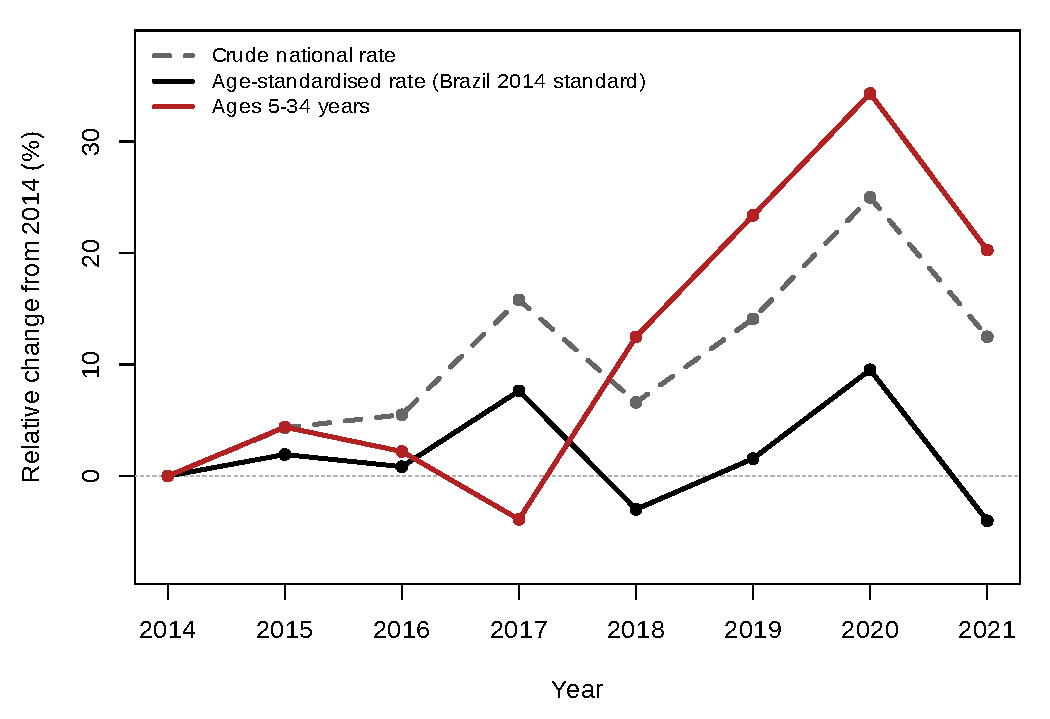
\includegraphics[width=0.85\textwidth]{figures/fig1_relative_change.pdf}
\caption{Relative change in each rate from its 2014 value, 2014--2021: crude national rate (dashed), age-standardised rate (Brazil 2014 standard, ages 7 or more) and rate at ages 5--34 years. Annual data; population from the IBGE 2018 projection.}
\label{fig:change}
\end{figure}

\clearpage
\begin{thebibliography}{9}
\bibitem{antunes2024} Brum M, Henz J, Boeira M, Soares S, Friedrich F, Pitrez PM. Recent increase in asthma mortality in Brazil: a warning sign for the public health system. J Bras Pneumol. 2024;50(5):e20240138. doi:10.36416/1806-3756/e20240138
\bibitem{sim} Ministério da Saúde (Brasil). Sistema de Informação sobre Mortalidade (SIM). Portal de Dados Abertos do SUS. \url{https://dadosabertos.saude.gov.br/dataset/sim}
\bibitem{ibge2018} Instituto Brasileiro de Geografia e Estatística. Projeção da População do Brasil e das Unidades da Federação, revisão 2018: população por idade simples, 2010--2060 (file projecoes\_2018\_populacao\_idade\_simples\_2010\_2060\_20201209.xls). \url{https://ftp.ibge.gov.br/Projecao_da_Populacao/Projecao_da_Populacao_2018/}. Accessed 1 October 2026
\bibitem{ibge2024} Instituto Brasileiro de Geografia e Estatística. Projeções da População, revisão 2024: população por idade simples (file projecoes\_2024\_tab1\_idade\_simples.xlsx). \url{https://ftp.ibge.gov.br/Projecao_da_Populacao/Projecao_da_Populacao_2024/}. Accessed 1 October 2026
\bibitem{antunescode} Brum M, et al. Analysis code accompanying reference~\cite{antunes2024}. GitHub repository, commit 8d527a5 (15 May 2024). \url{https://github.com/mobrant94/asthma_mortality}
\bibitem{ahmad2001} Ahmad OB, Boschi-Pinto C, Lopez AD, Murray CJL, Lozano R, Inoue M. Age standardization of rates: a new WHO standard. GPE Discussion Paper Series No. 31. Geneva: World Health Organization; 2001. \url{https://cdn.who.int/media/docs/default-source/gho-documents/global-health-estimates/gpe_discussion_paper_series_paper31_2001_age_standardization_rates.pdf}
\bibitem{mass} Venables WN, Ripley BD. Modern Applied Statistics with S. 4th ed. New York: Springer; 2002.
\bibitem{rcore} R Core Team. R: a language and environment for statistical computing. Vienna: R Foundation for Statistical Computing; 2024. \url{https://www.R-project.org/}
\end{thebibliography}

\end{document}
